\documentclass{article}
\usepackage{fancyhdr}
\usepackage[english]{babel}
\usepackage{indentfirst}
\usepackage[utf8]{inputenc}
\usepackage{graphicx}
\usepackage{caption}
\usepackage{subfigure}
\usepackage{multirow}
\usepackage{wrapfig}
\usepackage{media9}
\usepackage{hyperref}
\usepackage{float}
\usepackage{siunitx}
\usepackage{lastpage}
\usepackage{amsmath}
\usepackage{placeins}
\usepackage{multirow}
\usepackage{listings}
\usepackage{xcolor}
\usepackage{color}
\usepackage[titletoc]{appendix}
\usepackage[left=2cm, right=2cm, bottom=2cm]{geometry}

\graphicspath{ {./images/} }

\renewcommand{\familydefault}{\sfdefault}

\pagestyle{fancy}

\lhead{■■■ ■■■}
\chead{}
\lfoot{Page \thepage \space of \pageref{LastPage}}
\rhead{Candidate number ■■■, Centre number ■■■}
\rfoot{}

\begin{document}

\centerline{\textbf{{\huge The design and construction of a receiver for }}}
\centerline{\textbf{{\huge the acquisition of cost-effective satellite imagery}}}


\begin{figure}[H]
    \centering
    \includegraphics[scale=0.125]{imgs/setup full.jpg}
    \label{freq band image}
\end{figure}

\centerline{\textbf{{\Large ■■■ ■■■}}}

\centerline{\textbf{{\Large March 2023}}}

\newpage

\tableofcontents

\newpage


\section{Introduction}
    \begin{itemize}
        \item[] Satellites are essential tools for scientific research, national security, and commercial applications. They provide valuable data and images that can be used for a variety of purposes. Despite the high cost of launching and maintaining satellites, the benefits they provide make them an indispensable tool for humanity's continued exploration and understanding of the universe.

        This report aims to provide an overview of the use and development of satellites as well as summarise my project to design and build a receiver to gain affordable satellite images. 

        Satellites are artificial bodies created by humans and placed in orbit around the Earth or other space bodies to fulfil their missions. This paper discusses the different types of satellites, their purposes, and the instruments used to equip them for their missions. Additionally, it addresses the economic considerations of launching and maintaining satellites.

        \item[] \text{\bf Project aims}
            \begin{itemize}
                \item To design and build a receiver.
                \item To collect data to produce satellite images with the goal of high enough resolution images to enable future weather prediction. 
                \item To produce clear instructions on the design requirements and
                \item Evaluate the limitations and successes of the images collected. 
            \end{itemize}
        \item[] \text{\bf My objectives were to}
            \begin{itemize}
                \item To research and identify the necessary equipment for receiving satellite imagery
                \item To develop programming skills necessary for processing and analyzing the received satellite data
                \item To conduct experiments to optimize the satellite receiver and improve the quality of the received images.
                \item To document and explain the step-by-step instructions for receiving and processing satellite imagery
                \item To evaluate the cost and effectiveness of the homemade satellite receiver compared to commercially available alternatives
    
            \end{itemize}
    \end{itemize}

    
    
\section{Satellite imagery}
    \subsection{Satellites?}
        \begin{itemize}
            \item[] One of the most significant applications of satellites is their use for imaging the Earth's surface. By capturing high-resolution images of the planet, satellites provide valuable information to scientists, governments, and businesses. The images captured by satellites are used for a variety of purposes, including weather forecasting, resource management, and national security. A Satellite is a human made artificial body placed in an orbit around the earth or other space body in order to fulfill its mission. They come in different sizes (from 10 cm to 108 m) and have various purposes. Some of the most popular are NASA's\footnote{National Aeronautics and Space Administration} \textbf{Hubble} Space Telescope and ISS\footnote{International Space Station}
            
        \end{itemize}
    \subsection{Purpose of Satellites}
        \begin{itemize}
            \item[] Satellites can have one or multiple missions, depending on their purpose. Some of the most common missions of satellites include Earth surveillance, monitoring of the Sun, and exploration of other celestial bodies outside our solar system. Satellites can also be used for signal re-transmission or reception.
            \item[] To accomplish their missions, satellites are equipped with a range of instruments, including antennas, transmitters, and optical radiometers, such as visible light cameras. These instruments enable satellites to capture and transmit images and data to Earth.
            \item[] The cost of launching and maintaining satellites can be significant. While the cost of launching a satellite is decreasing, it is still expensive. As a result, it is economically unwise to call a repair crew to service a satellite. Therefore, satellite designers and manufacturers must ensure that their satellites can operate for as long as possible, sometimes for 30+ years.
            \begin{figure}[H]
                \centering
                \includegraphics[scale=0.3]{imgs/rocket-launch-costs-trend.jpg}  
                \caption{Projection of launch costs to low Earth orbit, 1980-2100 \cite{1}}
            \end{figure}
        \end{itemize}
    \subsection{Placing satellites in orbit.}
        \begin{itemize}
            \item[] The role of space agencies in satellite construction and deployment is significant, given the high cost and complexity of building and launching satellites. These agencies provide opportunities for various organizations to access the orbit and execute missions in space. NASA, the first space agency, remains a prominent player in the field, while private companies like SpaceX have become increasingly popular in recent years.
            \item[] It is evident\cite{2} that satellites, even small ones, are expensive, and the paper highlights the importance of careful planning and construction. This report also highlights the role of space agencies in facilitating satellite missions and providing opportunities for third-party  payloads.
            \item[] \textbf{The role of Space Agencies}

            \item[] Constructing a satellite is a complex task that requires significant resources and expertise, making it impossible for a single individual to accomplish. Thus, space agencies exist to plan and execute satellite missions. These agencies can be either private or government-based and have the capability to launch satellites into orbit. Additionally, they provide opportunities for third parties to place their payloads on the orbit.
            
            \item[] The first space agency was the United States' National Aeronautics and Space Administration (NASA), established in 1958. Three years prior, in 1955, the USSR had created a space program rather than an agency, known as the Soviet Space Program. Since then, numerous space agencies have emerged worldwide, with private companies like SpaceX, established in 2002, becoming increasingly popular.



        \end{itemize}
    \subsection{Active and Inactive space programs involving satellites}
        \begin{itemize}
            \item[] Satellite programs have now been around for more than six decades, and some have continued to serve various purposes, ranging from research to global positioning systems. The ISS, a multinational space station, is a prominent example of a satellite program used primarily for research in microgravity and earth observation. The Hubble Space Telescope has provided humanity with high-quality multi-spectrum pictures of far galaxies, and the GPS enables users to pinpoint their location with ease. These satellite programs are just a few examples of the many programs that have contributed significantly to human advancement and will likely continue to do so in the future.

            \item[] \textbf{Examples of such satellite programs include}
            \begin{itemize}
                \item International Space Station (ISS) -- This multinational space station was established in collaboration with NASA, (Roscosmos, JAXA\footnote{Japan Aerospace Exploration Agency}, ESA\footnote{European Space Agency}, CSA\footnote{Canadian Space Agency}) primarily used for various types of research in micro gravity and earth observation.
                \item Hubble Space Telescope -- NASA launched this versatile telescope in 1990, and it has since provided humanity with high-quality multi-spectrum pictures of far galaxies.
                \item Global Positioning System (GPS) Formerly known as NAVSTAR GPS, the system was launched in the 1980s and involves a belt of satellites around the earth. It enables users to pinpoint their location by calculating the delay between each satellite signal. With at least three satellites sending a signal, a pyramid could be modelled with one of the vertices being the user.
            \end{itemize}
        \end{itemize}
    \subsection{What is Orbit?}
        \begin{itemize}
            \item[] When considering how to put a satellite in orbit, the first idea that comes to mind is to leave it in the exosphere, outside the atmosphere. However, this method is not practical since the satellite will fall due to the Earth's gravity.
            \begin{figure}[H]
                \centering
                \includegraphics[scale=0.2]{imgs/Reaching_orbit_pillars.png}  
                \caption{Overcoming gravitational force through orbiting \cite{3}}
                \label{orbit1-img}
            \end{figure}
            \item[] \parbox[t]{\dimexpr\textwidth-\leftmargin}{
                \begin{wrapfigure}{R}{0.45\textwidth}
                    \vspace{-\baselineskip}
                    \includegraphics[width=\linewidth]{imgs/Communication-satellites-orbiting-the-Earth-in-geostationary-orbits-GEO-Low-Earth.png}
                    \caption{Different orbits \cite{5}}
                \end{wrapfigure}
                There are various types of orbits that can be used to keep an artificial body near the Earth:
                \begin{itemize}
                    \item LEO, or Low Earth Orbit, is the closest orbit to Earth, with an altitude of less than 1000 km. Satellites in LEO always travel around the Earth on different paths, which allows for full coverage of the Earth's surface. This type of orbit is ideal for weather surveillance
                    \item GEO, or Geostationary Orbit, is an orbit in which the satellite stays in one place above the equator line, travelling at the exact same speed as the Earth rotates. This makes the satellite appear stationary in the sky, making it perfect for signal re-transmission, television, and communication
                    \item HEO, or Highly Elliptical Orbit, follows an elliptical path with the closest point (perigee) at 1000 km and the furthest point (apogee) at 35,000 km. This type of orbit is useful for sectoral Earth observation, as the satellite's ground track will appear to follow a figure-eight pattern.


                \end{itemize}
                }
        
           
        \end{itemize}
    % \subsection{Orbit prediction}
    %     \begin{itemize}
    %         \item[] 
    %     \end{itemize}

\section{Signal reception}
    \subsection{What is signal?}
        \begin{itemize}
            \item[] A signal is defined as an electromagnetic wave that carries radiant energy and travels through space\cite{6}. The electromagnetic field is responsible for generating these waves. This wave is composed of a specific frequency and strength, which distinguish it from other types of waves, such as light, radio, and Wi-Fi. To receive satellite signals, it is essential to consider the polarisation of the wave, which refers to the way the wave is displaced as it travels through space.

            \begin{figure}[H]
                \centering
                \includegraphics[scale=0.325]{imgs/polar.jpg}
                \caption{Different types of polarisation on graph \cite{6}}
            \end{figure}
            
            In this project, I have chosen for the main focus will be on the Right Hand Circular Polarized [RHCP] signal, which is commonly used by most satellites due to its high resilience to interference. However, another crucial property of a signal is its frequency. 

            \item[] Different communication needs require different frequencies. For instance, a powerful 3kHz signal would be suitable for long-range communication with trade ships, while 2.4 GHz is better for shorter distances but can encode more data and requires less energy to transmit, making it ideal for Wi-Fi
            
            \begin{figure}[H]
                \centering
                \includegraphics[scale=0.55]{imgs/radio-frequency-bands.png}
                \caption{Band of frequencies use \cite{11}}
                \label{freq band image}
            \end{figure}
            
            LRPT\footnote{Low Resolution Picture Transmission} and APT\footnote{Analog Picture Transmission} modules installed on the weather satellites transmit at around 137.1 MHz. We will have to take this into account when producing an antenna as incorrectly tuned one will have much worse reception.

            \item[] In today's world, there is a large number of devices that use radio waves to communicate, such as phones, PCs, and tablets, but there is only a limited bandwidth of frequencies that can be economically used. With a fixed rate of oscillations (baud rate) and limited transmission range, it only takes a few dozen devices to start significantly interfering with each other, such as in a public cafe where Wi-Fi is slow due to many users "talking over" each other when communicating with the access point. So, how was this problem solved?

            \textbf{Modulation} is a special method of adding data to signal by using its multiple physical properties like amplitude or phase.

            \begin{figure}[H]
                \centering
                \includegraphics[scale=0.55]{imgs/DigitalMod_pt1_fig1_Digital_modulation_waveforms_659x601.jpg.png}
                \caption{Modulation methods \cite{7}}
                \label{mod-type-img}
            \end{figure}

            
            
            \item[] \textbf{The impact of modulation}
            
            \item[] When considering our goal of building a weather satellite imagery system, the concept of "modulation" becomes important. In order to receive signals from the Meteor-M N2 satellite, I will need to understand the Low Rate Picture Transmission (LRPT) system that it uses. 

            \item[] LRPT\cite{7} is a digital transmission system used for image delivery from orbiting satellites. The Meteor-M N2 satellite transmits a 120 kHz signal at 72,000 symbols per second using Quadrature Phase-Shift Keying (QPSK) modulation. QPSK uses phase shift as a modulation method.

            \begin{figure}[H]
                \centering
                \includegraphics[scale=0.15]{imgs/qpsk-symbols.png}
                \caption{QPSK waveform \cite{8}}
                \label{mod-type-img}
            \end{figure}

            In a communication system, the modulation method used is crucial to determine the data rate and reliability of the signal. Quadrature Phase-Shift Keying [QPSK] is one of the most commonly used modulation methods in digital communication systems. QPSK uses four phases, each 90 degrees apart, making it possible to encode 4 bits at once (00, 01, 10, and 11). This approach allows for a higher data rate with little to no increase in error probability. In fact, there are no significant disadvantages to using QPSK modulation, except for the relative modulation complexity.



            \begin{figure}[H]
                \centering
                \includegraphics[scale=0.8]{imgs/Quadrature-Phase-Shift-Keying-Waveform.jpg}
                \caption{QPSK waveform \cite{8}}
                \label{mod-type-img}
            \end{figure}
            
            
        \end{itemize}
  \subsection{Antenna design}
        \begin{itemize}
            \item[] To receive the RHCP signal used by the satellite, a specific type of antenna is required that can effectively receive this type of polarization. Additionally, since the satellite will be moving and motorized tracking is not an option, the antenna design should be able to receive the signal from a moving source, making an omnidirectional antenna the ideal solution.


            \item[] The dipole is a simple and affordable omnidirectional antenna design that consists of two wires at a length or half-length of the signal frequency protruding from a conductor base. This antenna design is a good starting point for our project, and we can improve its performance by tuning it to the specific frequency of the signal we want to receive.

        \begin{figure}[H]
            \centering
            \includegraphics[scale=0.4]{imgs/Dipole simple.jpeg}
            \caption{Simple half-wavelength dipole design\cite{10}}
        \end{figure}

        The target satellite is going to be moving overhead from south to north horizons as seen on diagram \ref{polar-axis}.

        \begin{figure}[H]
            \centering
            \includegraphics[scale=0.1333]{imgs/Polar track.jpeg}
            \caption{Overhead pass of satellite on polar diagram (self drawn)}
            \label{polar-axis}
        \end{figure}

        The dipole antenna could be configured in 3 main ways
        \begin{itemize}
            \item Wire length -- The target frequency of the satellite is 137.1 MHz. Using the formula
            \begin{align}
                & L = \frac{143}{f}
                & l = \frac{L}{2}
            \end{align}
            where L is the length of the antenna in meters and f is the frequency in MHz, we can calculate the length of one of the two antenna elements. 
            \begin{align}
                & L = \frac{143}{137.1} = \SI{1.043}{\metre}
                & l = \frac{1.043}{2} = \SI{0.5215}{\metre} = \SI{52.15}{\centi\metre}
            \end{align}
            \item Wire angle and elevation: Since the satellite signal is Right Hand Circularly Polarised (RHCP), there is a particular variation of dipole that is good at receiving it – the V-Dipole. 
            \item[] The V-Dipole is a simple dipole with both antenna legs bent at a specific angle. The optimal angle has been reported by Bouwens\cite{22} a member of the RTL-SDR community. Through an electromagnetic simulation in the Numerical Electromagnetic Code (NEC) software, a program, which predates modern computers, he determined the antenna designs, where the parameters of the wire, ground, and current were specified. He used a simplified model of the dipole to determine the optimal angle.

            \begin{figure}[H]
                \centering
                \includegraphics[scale=0.333]{imgs/arno-v-dipole.png}
                \caption{Schematic of the V-dipole model Arno has used \cite{12}}
                \label{dipole-simple-img}
            \end{figure}

            Arno\cite{12} determined that "The effect of the V-angle seems quite small in this view of the radiation pattern." However, the elevation angle has a significant impact on the strength of the received signal from the overhead satellite. According to Arno's simulation\cite{12}, elevation influences the radiation pattern of the antenna 13, which is the strength at which the antenna receives a particular signal from a specific angle.
            
            \begin{figure}[H]
                \centering
                \includegraphics[scale=0.5]{imgs/5and1mElevation.png}
                \caption{"Gain [dB], $30^{\circ}$ elevation, $\lambda/2$ above average ground" \cite{13}}
                \label{arno-elev}
            \end{figure}

            According to Arno's simulation[12], the optimal antenna height for receiving the satellite signal depends on the elevation angle of the satellite. Arno suggests that "when the satellite is at an elevation > 45◦, it’s best to have the antenna at about 0.5 m. From 15-45◦, 1 m seems to give good gain." This means that for the first and last third of the pass, it is better to position the antenna 1 m above the ground, and for the time when the satellite is directly above, 0.5 m would be the best height.

            Citing Arno once again "when the satellite is at an elevation $>45^{\circ}$, it’s best to have the antenna at about $\SI{0.5}{\metre}$. From 15-$45^{\circ}$, $\SI{1}{\metre}$ seems to give good gain." Meaning that for the first and last third of the pass it is better to position antenna $\SI{1}{\metre}$ above the ground and for the time when the satellite is directly above $\SI{0.5}{\metre}$ would be the best.
            
        \end{itemize}

    \end{itemize}
        
    \subsection{How professional ground stations do it?}
        \begin{itemize}
            \item[] At the professional side of things, scientific ground stations receive and transmit signals for research or commercial purposes. At a higher level, more high-quality equipment is available, like high-voltage transmitters and more sensitive reception modules. Along with powerful transmitters, huge satellite dishes are used. The bigger the dish, the more precise the pointing should be; that is why bigger directional parabolic antennas require high precision. This could be achieved by motorized tracking, which is possible to obtain, but it is very expensive. Location of the ground station plays an important role as well. Modern cities are polluted with radio interference, so it is important to reduce it. Remote deserts with a 180 degree view of horizons or high mountains are a perfect fit; this is going to influence the choice of my location for my satellite receiver. 



            \begin{figure}[H]
                \centering
                \includegraphics[scale=0.55]{imgs/antenna array.jpg}
                \caption{Owens Valley Radio Observatory \cite{9}}
                \label{dish-array-img}
            \end{figure}
            
        \end{itemize}
    \subsection{Sourcing appropriate equipment.}
        \begin{itemize}
            \item[] The amateur radio community has grown tired of using only high-spec equipment that can be expensive, and they have made efforts to make ham radio more accessible, leading to the development of Software Defined Radio (SDR). The most popular amateur radio dongle is the RTL-SDR 15, which costs £36. However, I have found cheaper alternatives from NooElec that can go as low as £28 and a full kit that includes a multipurpose antenna from Amazon UK.

                    
                    
        \begin{figure}[H]
            \centering
            \begin{subfigure}{0.5\textwidth}
                \centering
                \includegraphics[width=.55\linewidth]{imgs/rtl1.jpg}
                \caption{RTL-SDR USB dongle \cite{14}}
                \label{fig:rtl1}
            \end{subfigure}%
            \begin{subfigure}{0.5\textwidth}
                \centering
                \includegraphics[width=.55\linewidth]{imgs/rtl-kit.jpg}
                \caption{Antenna kit \cite{14}}
                \label{fig:rtl-kit}
            \end{subfigure}
            \caption{Antenna kit [15]: and readily available RTL-SDR configurations}
            \label{fig:test}
        \end{figure}

        \end{itemize}
    
    \subsection{Equipment needed}
    \begin{itemize}
        \item[] \textbf{Essensials:}
        \item Laptop -- In my experience, getting a good reception at home is unlikely, so I'll need to head outdoors. I'll be using a laptop running Windows or Linux with at least one hour of battery charge and a USB port. Of course the cost of the laptop is not considered in the final cost as it is assumed that it is already present.
        \item Receiver -- I prefer to use the classic RTL-SDR, but the NooElec or HackRF One could also be suitable options. NooElec being considerably cheaper does have a cost advantage, however it is slightly limited in the receiving range of spectrum (only 1.75 GHz, unlike 2.2 GHz in RTL-SDR). HackRF one is a good option too and has considerably better hardware (5.5 GHz and 40 Mhz active band) but it costs around £450. Overall RTL-SDR (£34) is a good middle ground in price and functionality that I need for the purposes of the project.
        Other things that I have included after the proper research
        \item[] \textbf{Upgrades:}
        \item Filters -- Even in remote areas, some radio interference can still be present, so I have decide to use frequency filters. I purchased mine from the RTL blog, including a low-frequency 2.6 kHz filter and an FM radio filter  for the 88-108 MHz range (£18 a piece). These filters greatly improve the strength of the receiving signal by blocking all of the unnecessary interference at the physical level.
        \item Low Noise Amplifier -- LNA is an amplifier that increases the amplitude of weak signals. I'm using the Wideband LNA from RTL-SDR Blog, which came in a bundle with the filters. (20£ separately) It allows for the low intensity signals such as satellite signal to be picked up by the receiver, this however increases the overall noise level as well as other neighboring signals on the spectrum, so it is beneficial to tweak the sensitivity to achieve the best noise to signal contrast.
        \item Location -- Although it's possible to receive signals from the balcony or window of an apartment building, an open area with little obstruction to the sky, ensuring that the passing satellite is visible from N to S horizons would be preferable. That is why I choose the roof as a primary location instead of an open field. which is likely to have obstructions such as surrounding forestry.
        \item Mount -- To adjust the antenna's height throughout the pass, I'll be using a tripod that I was able to borrow for the time of capture. Hand-holding the antenna is also possible, however it is not recommended not only because it is tiring but also slight hand shake makes the dipole's whiskers wiggle a little, this decreases the clarity of the signal. In addition to that, when mounted it is much easier to control the height of the antenna from the ground, the rotating handle allows for precise adjustments which are needed to maximise the reception time as mentioned by the Arno's research.
        \item Antenna -- I need to produce a dipole using the described design. If I have the necessary resources and tools such as copper wire, wooden planks and a soldering iron, I can manufacture it from scratch, but I'll be using the one from the kit I purchased with the receiver. Cost wise DIY is cheaper, all of the required components could be found in the household or in college workshop (about £7), however the kit antenna could be easily configured by adjusting the whiskers length, so it is preferred if multiple signal frequencies are going to be captured in a single session. The RTL kit includes a mount and a cord extender which allows to freely position the antenna independently from the receiver, however it is comparatively more expensive £24 on eBay.

        \item All of the mentioned costs could be summarised into this table
        
        \item[] \begin{tabular}{ |p{3cm}||p{3cm}|p{3cm}|  }
             \hline
             \multicolumn{3}{|c|}{\textbf{Total cost breakdown}} \\
             \hline
             Equipment & Is required? & Price (£)\\
             \hline
             Laptop & Yes & N/A\\
             RTL-SDR & Yes & 34\\
             AM FIlter & No & 18\\
             FM FIlter & No & 18\\
             LNA & No & 20\\
             Mount & No & 7\\
             
             \hline
             \multicolumn{3}{|c|}{\textbf{Cheapest configuration: £34}} \\
             \hline
             \multicolumn{3}{|c|}{\textbf{Full configuration £97}} \\
             \hline
            \end{tabular}

        \item[] £97 is a considerable sum of money, however a few things should be taken into account. Firstly, professional radio equipment could go into several thousand pounds just for the receiver, not including antenna or filters. That is comparatively more expensive than an amateur setup that will do exactly the same thing and would be much more portable than a bulky machinery that a professional radio equipment is. And secondly some of the costs such as antenna or mount could be omitted in case one already has such things, in my case I lent the tripod from my sister. All of the equipment mentioned was considered to be new, however there is no downside in using second hand from eBay or their platform, this could cut a couple of dozen pounds of a final cost.

        Overall I consider the price aspect to be met as £97 is a reasonable sum for a radio equipment.

    \end{itemize}

\section{Action!}
    \subsection{Setting up the reception station}
        \subsubsection{Laptop}
            \begin{itemize}
                \item[] My first step was to install RTL-SDR drivers. I found that the RTL Blog provided a step by step guide for this\cite{15}.
                \item[] From testing different drivers, I found that I very much preferred the ”Meteor LRPT Suite”[16]. This suite included all of the programs for the satellite imagery, but I will focused on using the SDR\# – software which I found to be  compatible with RTL-SDR and other sdrs. This particular version includes plugins for Meteor satellite that helped me to lock onto the signal and demodulate it on the fly.
                
                \begin{figure}[H]
                    \centering
                    \includegraphics[scale=0.475]{imgs/sdr-sharp.png}
                    \caption{SDR\# with Meteor plugin}
                    \label{img:sdr-sharp}
                \end{figure}

                \item[] For the decoding part I tested the recommend ”SatDump” from Altillimity’s GitHub page\cite{17} which has support for a very wide range of weather satellites and produces higher quality images that are not stretched unlike those produced by the older version of LRPTDecoder in the suite. As it is an open-source software distributed freely, a lot of community members regularly update the software to include the latest weather satellite decoders, so it is another plus.
                
                \begin{figure}[H]
                    \centering
                    \includegraphics[scale=0.45]{imgs/satdump.png}
                    \caption{SatSatDump GUI \cite{satdump}}
                    \label{img:satdump}
                \end{figure}
                
                \item[] ”Look4Sat” by Arty Bishop \cite{18}. has a simple interface and reliably predicts passes for selected satellites, more over the compass function enables user to point and see exactly where satellite passes in the sky. Unfortunately there is currently no alternative for the iOS devices so I decided to use Gpredict\cite{19} It is another satellite tracking and prediction software available for Windwos, Linux and MacOS. Gpredict has more functionality compared to mobile Look4Sat, it cam predict satellite passes several years into the future as well as a support for GEO stationary satellites.
                
                \begin{figure}[H]
                    \centering
                    \includegraphics[scale=0.2]{imgs/look4sat.png}
                    \caption{Look4Sat on Android}
                    \label{img:look4sat}
                \end{figure}
                
            \end{itemize}
        \subsubsection{Environment}
            \begin{itemize}
                \item[] As previously discussed, the choice of location for good reception is crucial. Although additional filters and amplifiers can be used, these cannot compete with the advantages of an open space in a field or on a roof. Through trial and error with my receiver, I discovered that that reception inside my building was next to nothing. I was fortunate to have access to the roof a 17-story apartment complex. This proved to be an excellent location for reception. The area had a nice elevated block with ladder access, providing a 360-degree view with no obstructions. Due to the location of the apartment block in the city, I found that filters were helpful in reducing radio interference. It should be noted that at high altitudes the gusts of wind become particularly strong, so it is important to always be ware of the surrounding to not fall as well as that I had an unfortunate accident during one of the first attempts, the receiver was blown away from the elevated block and fell down, the AM filter was damaged, the mounting head for the cable was bent and torn apart from the circuit, however serviceable, I was unable to use it anymore. 

                \begin{figure}[H]
                    \centering
                    \begin{subfigure}{0.3\textwidth}
                        \centering
                        \includegraphics[width=.95\linewidth]{imgs/roof2.jpg}
                        \caption{New capture location}
                        \label{fig:roof2}
                    \end{subfigure}
                \end{figure}
            \end{itemize}

        \subsubsection{Ground station}
            \begin{itemize}
                \item[] Once in location I began to position the antenna. I positioned all the equipment under a small border so it would not be blown away by the wind. 

                \begin{figure}[H]
                    \centering
                    \includegraphics[scale=0.1]{imgs/setup unassebled.jpg}
                    \caption{All the things we need}
                    \label{img:unassembled}
                \end{figure}

                \item[] The mount was chosen to be  a tripod that I borrowed. It was 40 cm in height and could be extended up to 1.1m. which provided to be an ideal range for the height adjustments.

                \begin{figure}[H]
                    \centering
                    \includegraphics[scale=0.075]{imgs/setup tripod.jpg}
                    \caption{Tripod with height adjustment}
                    \label{img:tripod}
                \end{figure}

                \item[] I used a multipurpose dipole antenna 26 from the RTL-SDR kit.

                \begin{figure}[H]
                    \centering
                    \includegraphics[scale=0.1]{imgs/setup dipole.jpg}
                    \caption{Multipurpose dipole}
                    \label{img:dipole}
                \end{figure}

                \item[] The whiskers were 55.4 cm each side and were set at a 60 degree angle.

                \begin{figure}[H]
                    \centering
                    \begin{subfigure}{\textwidth}
                        \centering
                        \includegraphics[width=.75\linewidth]{imgs/setup whiskers.jpg}
                        \caption{Whiskers}
                        \label{img:whiskers}
                    \end{subfigure}%
                    \begin{subfigure}{\textwidth}
                        \centering
                        \includegraphics[width=.75\linewidth]{imgs/setup angle.jpg}
                        \caption{V-Dipole}
                        \label{img:vdipole}
                    \end{subfigure}
                    \label{fig:test}
                \end{figure}

                \item[] After the antenna is configured it was mounted on the tripod. With a general mount screw for camera,

                \begin{figure}[H]
                    \centering
                    \includegraphics[scale=0.1]{imgs/setup low.jpg}
                    \caption{Antenna mounted on tripod}
                    \label{img:mount}
                \end{figure}
                
        \end{itemize}
        
    \subsection{Receiving the signal}
        \begin{itemize}
            \item[] Once ready I was just in time for the NOAA satellite pass. For this pass I decided to not adjust the height if the tripod to measure the increase in performance in the next pass. The receiver was connected to the laptop via USB extender I found and laptop had SDR\# up and running in record mode. Once the NOAA pass began I started to notice the slight signal fluctuations in spectrum view.

            \begin{figure}[H]
                    \centering
                    \includegraphics[scale=0.4]{imgs/noaa-pass.jpg}
                    \caption{First clear NOAA signal}
                    \label{img:mount}
                \end{figure}

            \item[] I recorded the spectrum during the entirety of the satellite pass which was about 19 minutes, however the length of distinguishable signal was only 13 minutes. It was evident that nearing the horizon the quality of the signal decreased significantly. In the next pass of the METEOR satellite I made an adjustment to the tripod according to Arno's findings. During the start of the pass I adjust the tripod to 1m from ground, then as the satellite approached the 90 degree mark, being just above my head I proportionately decreased the height back to 50cm, and then back to 1m as satellite was reaching the other end of the horizon. Having recorded the spectrum I noticed that the total signal duration was nearing 18 minutes, which is a clear improvement comparing to 13 minutes. As later experiments with height indicated the data decoded with no height adjustment was about 65 Megabytes in size, whereas with height adjustment it was approaching 90 Megabytes.

            \item[] As for the equipment, I initially misplaced the LNA and it was facing the wrong way, I later noticed that the SDR\# did not pick it up and had no LNA option active, so I reassembled the receiver. Overall the LNA significantly improves the overall signal strength however it introduces increased noise floor to the spectrum. Variable from time to time I made necessary adjustments to the Gain setting in the SD\# so that optimal noise to signal contrast was preserved.

            \item[] Having recorded 4 passes over the course of 1:30 hours, my laptop battery was depleting, so I returned to home and started the decoding process. SatDump was easy to use, having selected the appropriate satellite type I loaded the baseband recording of my METEOR passes. It took about 4 minutes to decode and stretch the image as transmitted images are deformed because of the wide lens on the satellite. The overall result was pretty good, the signal carried 3 channels of data -- green, blue and infrared, combining the data and adjusting the contrast I obtained a colourful picture. Considering it was night time not much detail could be seen, but it was evident that the picture quality increased dramatically.

            \begin{figure}[H]
                    \centering
                    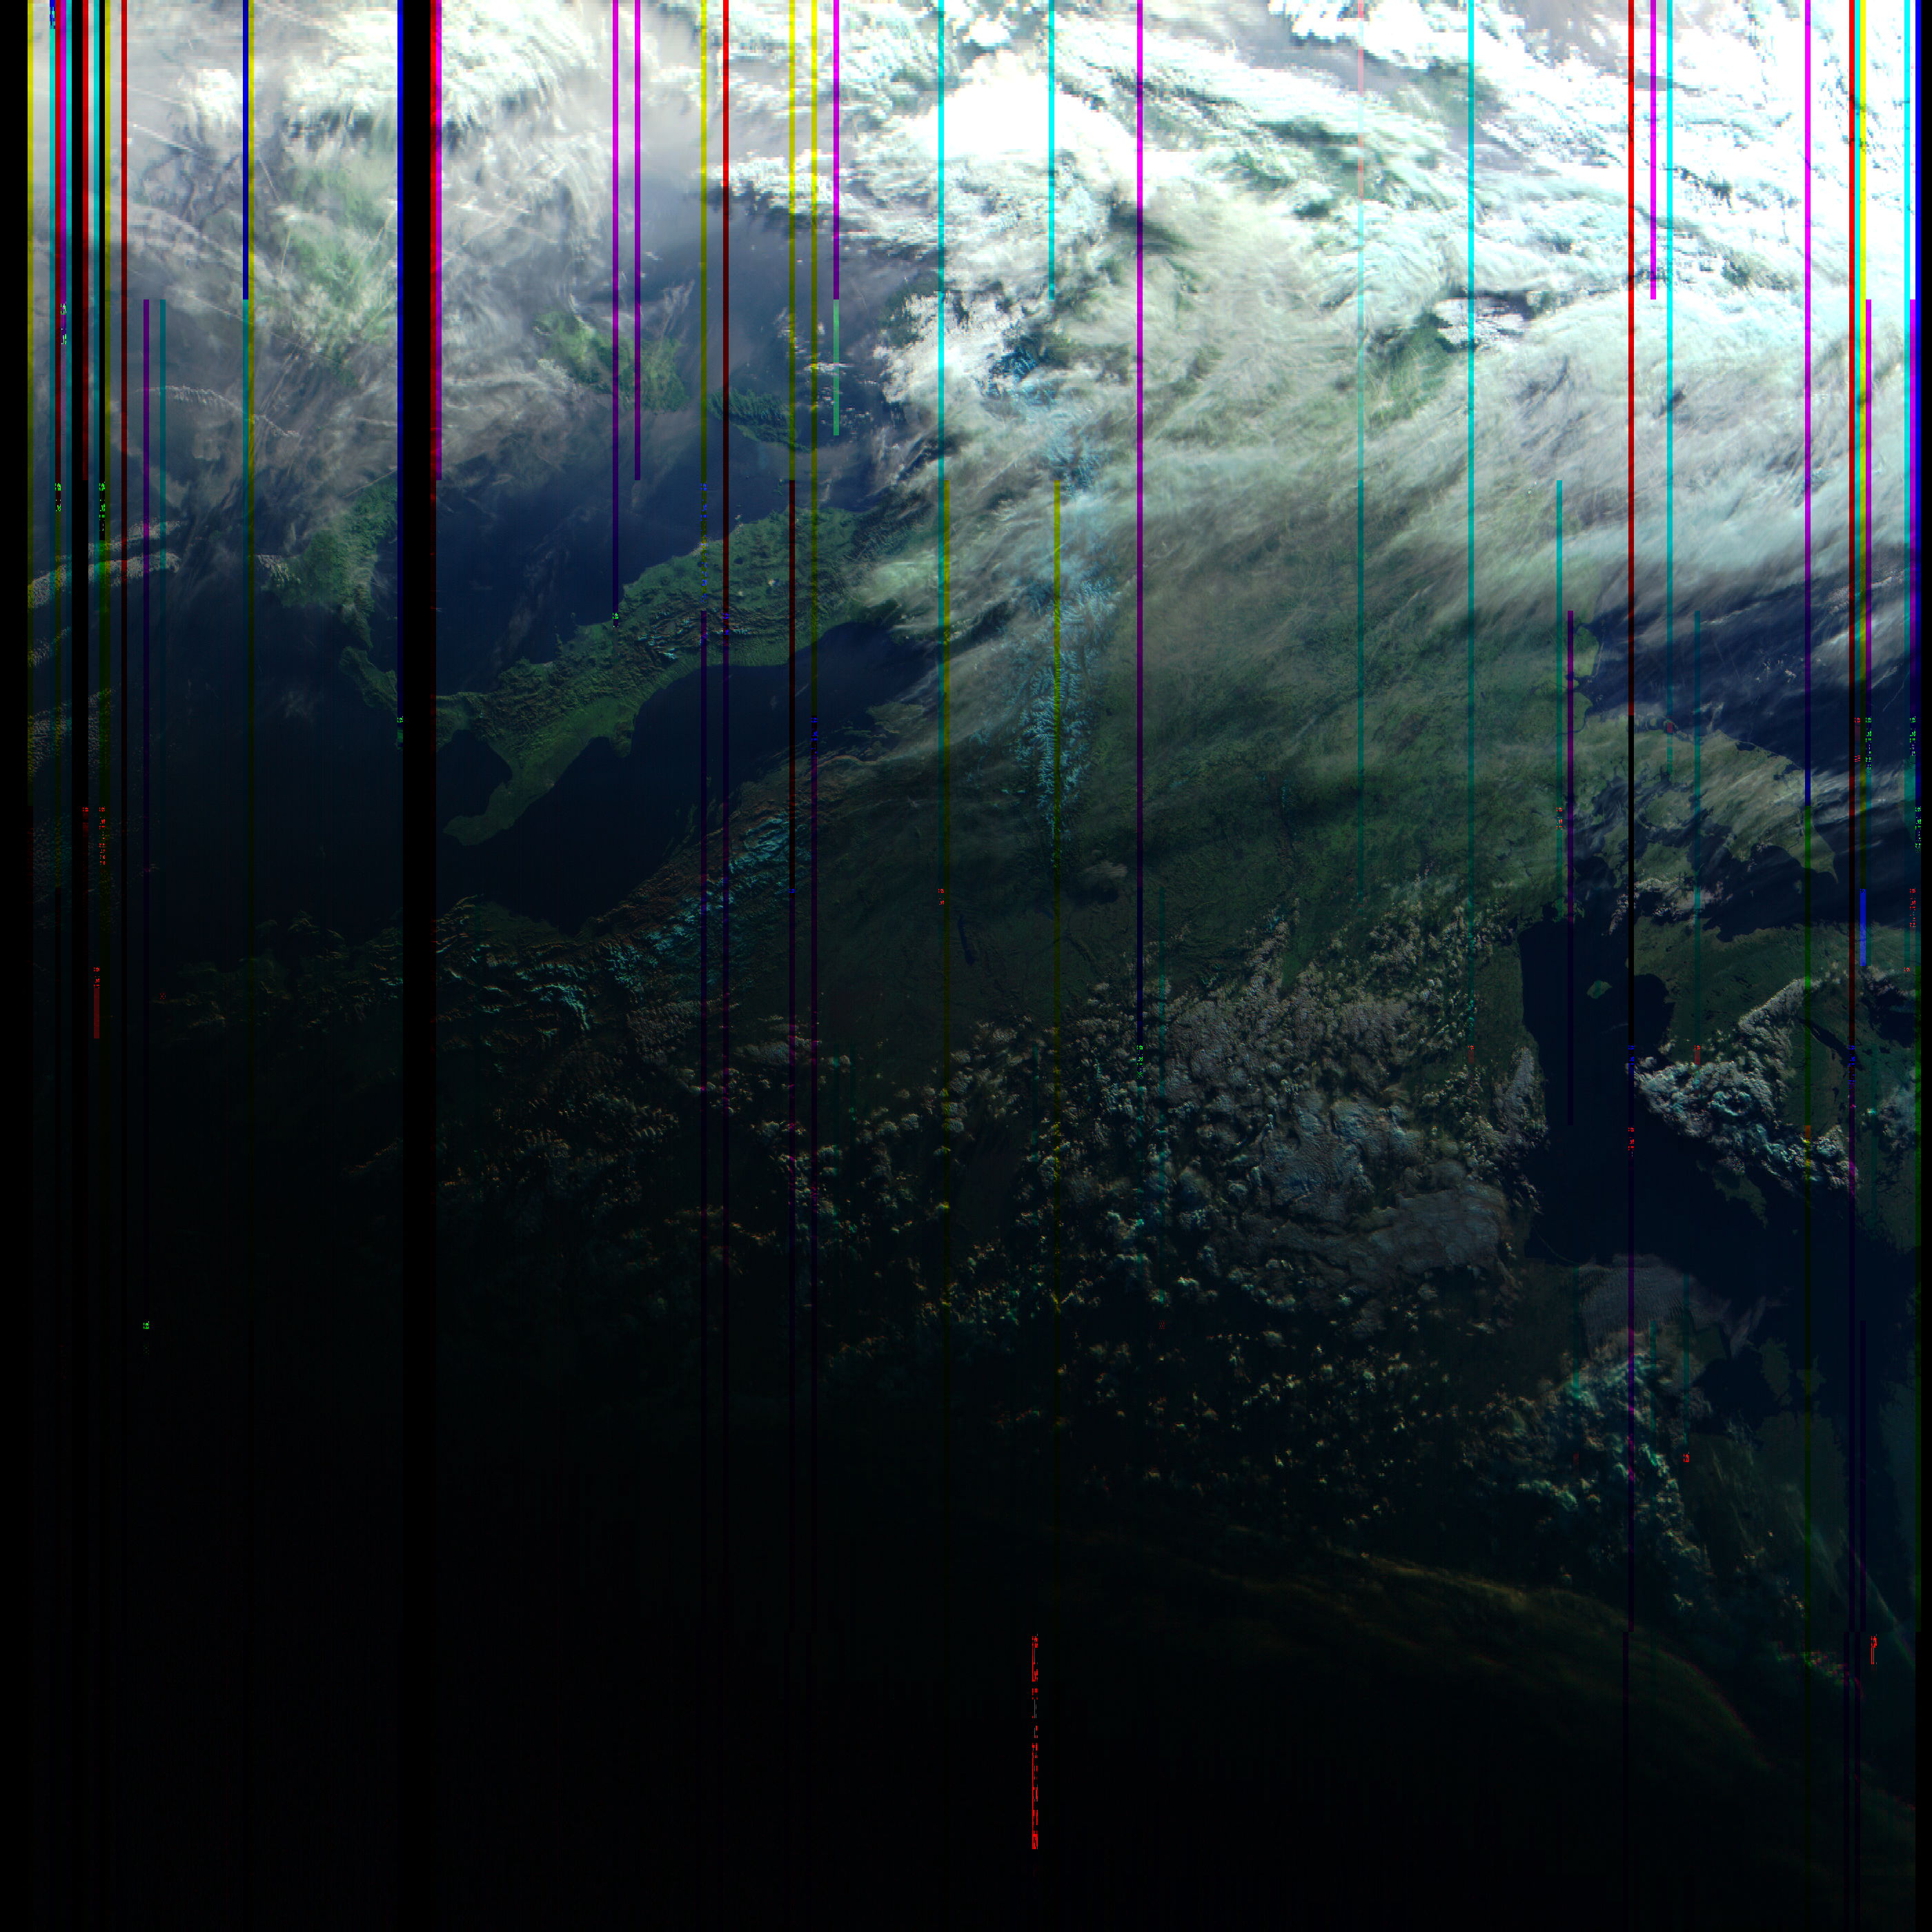
\includegraphics[scale=0.2]{imgs/Meteor Apr 12.png}
                    \caption{Meteor night picture of South Europe}
                    \label{img:mount}
                \end{figure}

            \item[] Next up was NOAA recording. It was an analog signal so it would have considerably lower level of detail, but good nonetheless. For analog signal that NOAA satellite transmit I used the LRPT Decoder that was in the Suite mentioned. The image transmit ed had only two channels available -- grayscale and infrared. I artificially added colours to the picture.

            \begin{figure}[H]
                    \centering
                    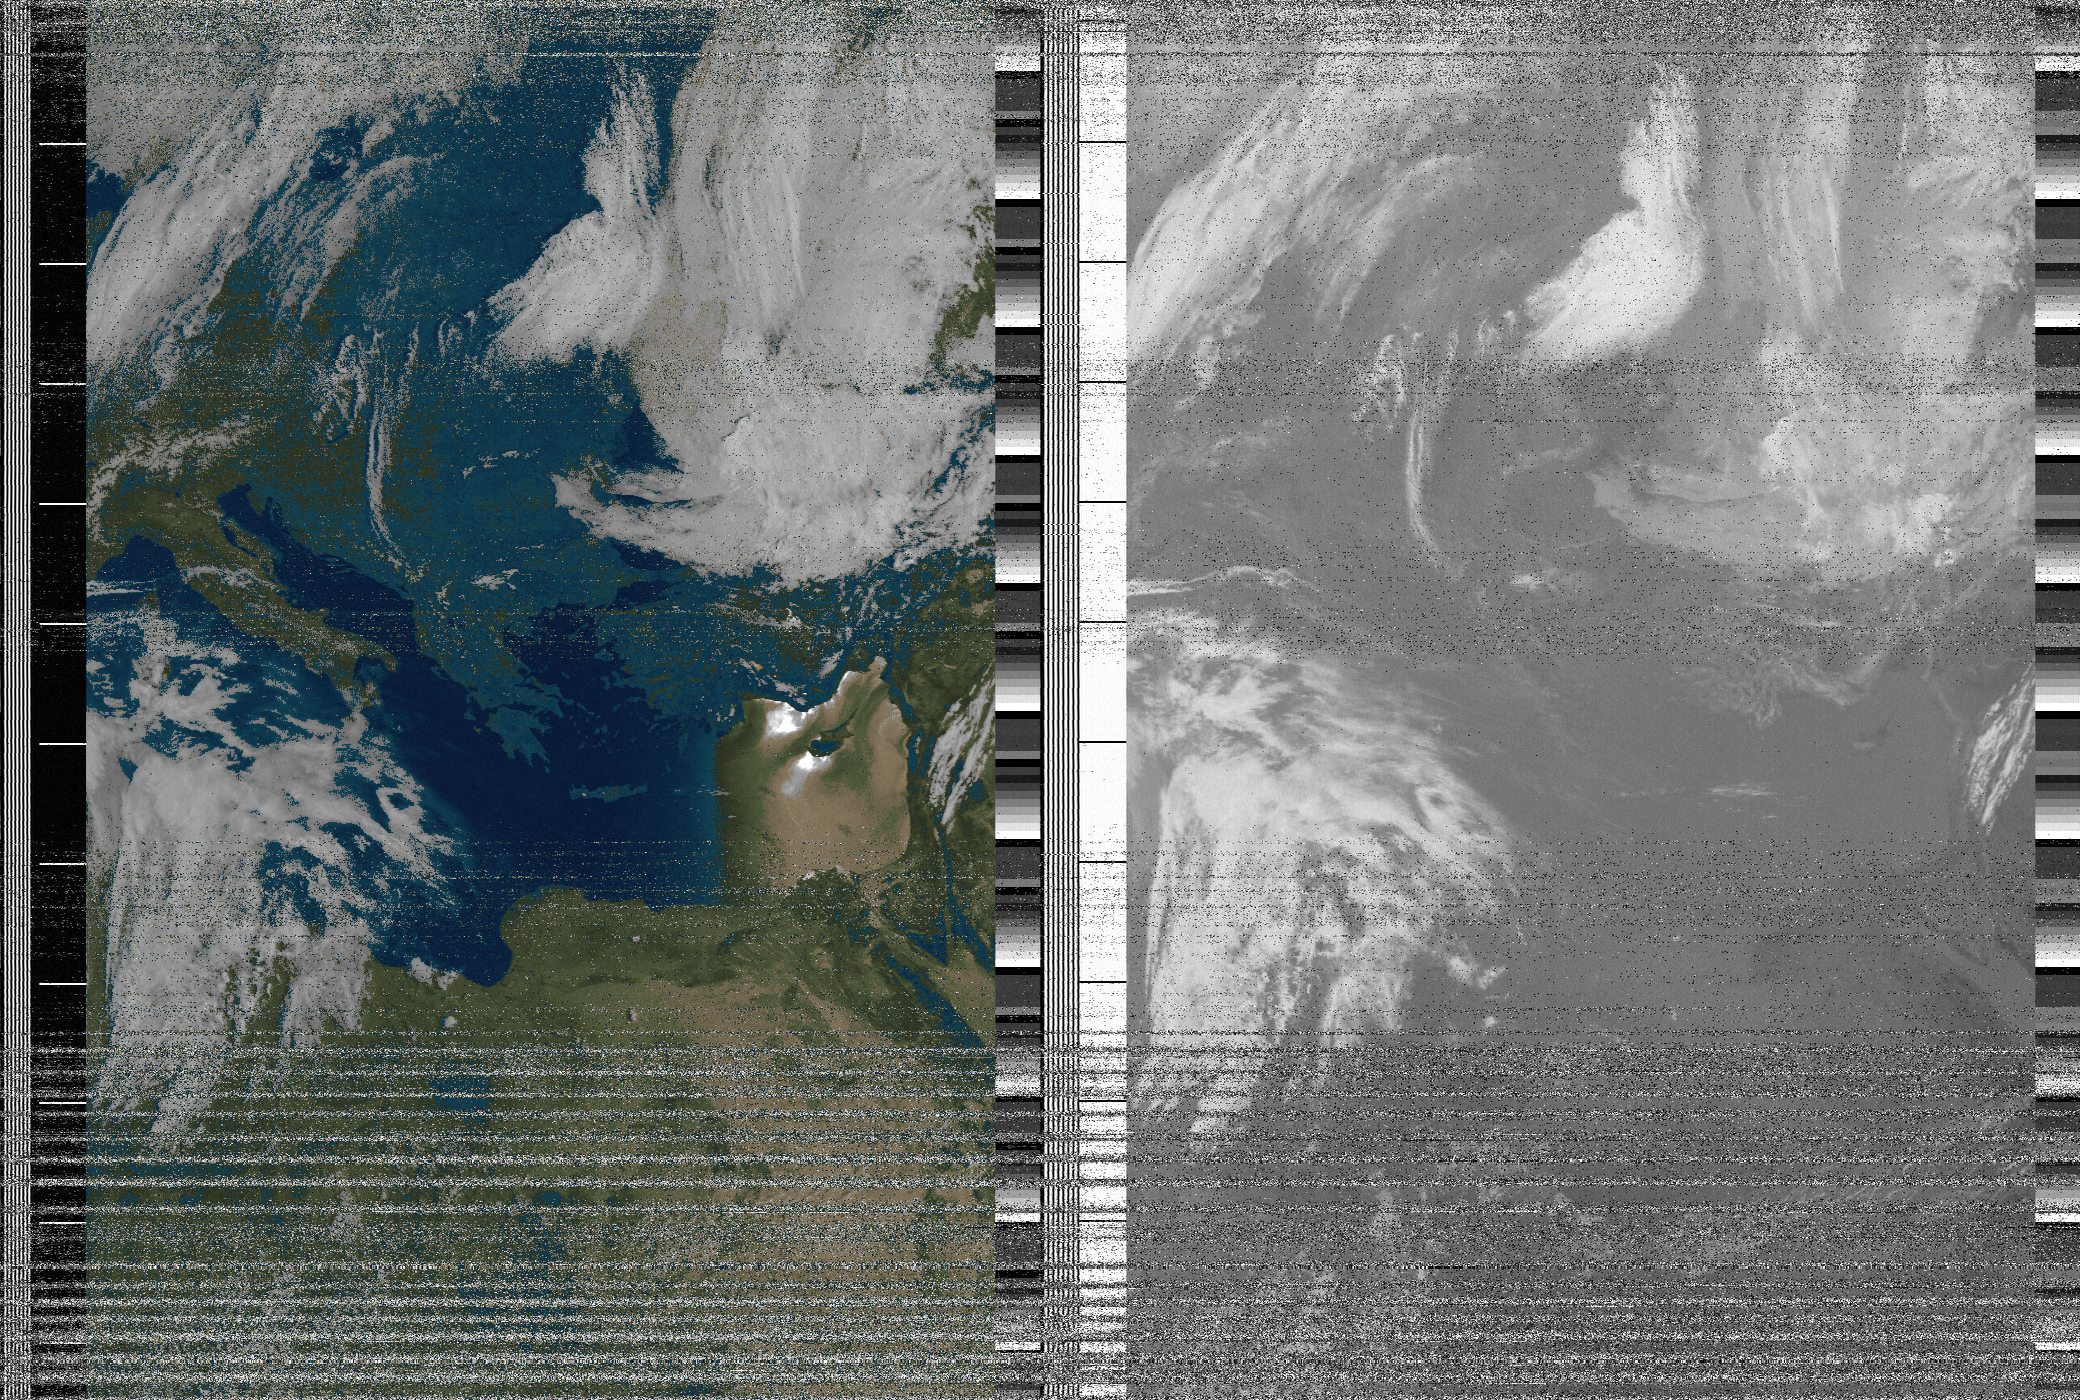
\includegraphics[scale=0.2]{imgs/8.png}
                    \caption{Artificially coloured NOAA image}
                    \label{img:mount}
                \end{figure}   
    
        \end{itemize}
    \subsection{Possible use case}
        \begin{itemize}
            \item[] Having successfully received and decoded image from the weather satellite one could possibly start making their own weather predictions. Once I went back to UK I captured a couple of more passes and made a temperature composition of a UK region.

            \begin{figure}[H]
                    \centering
                    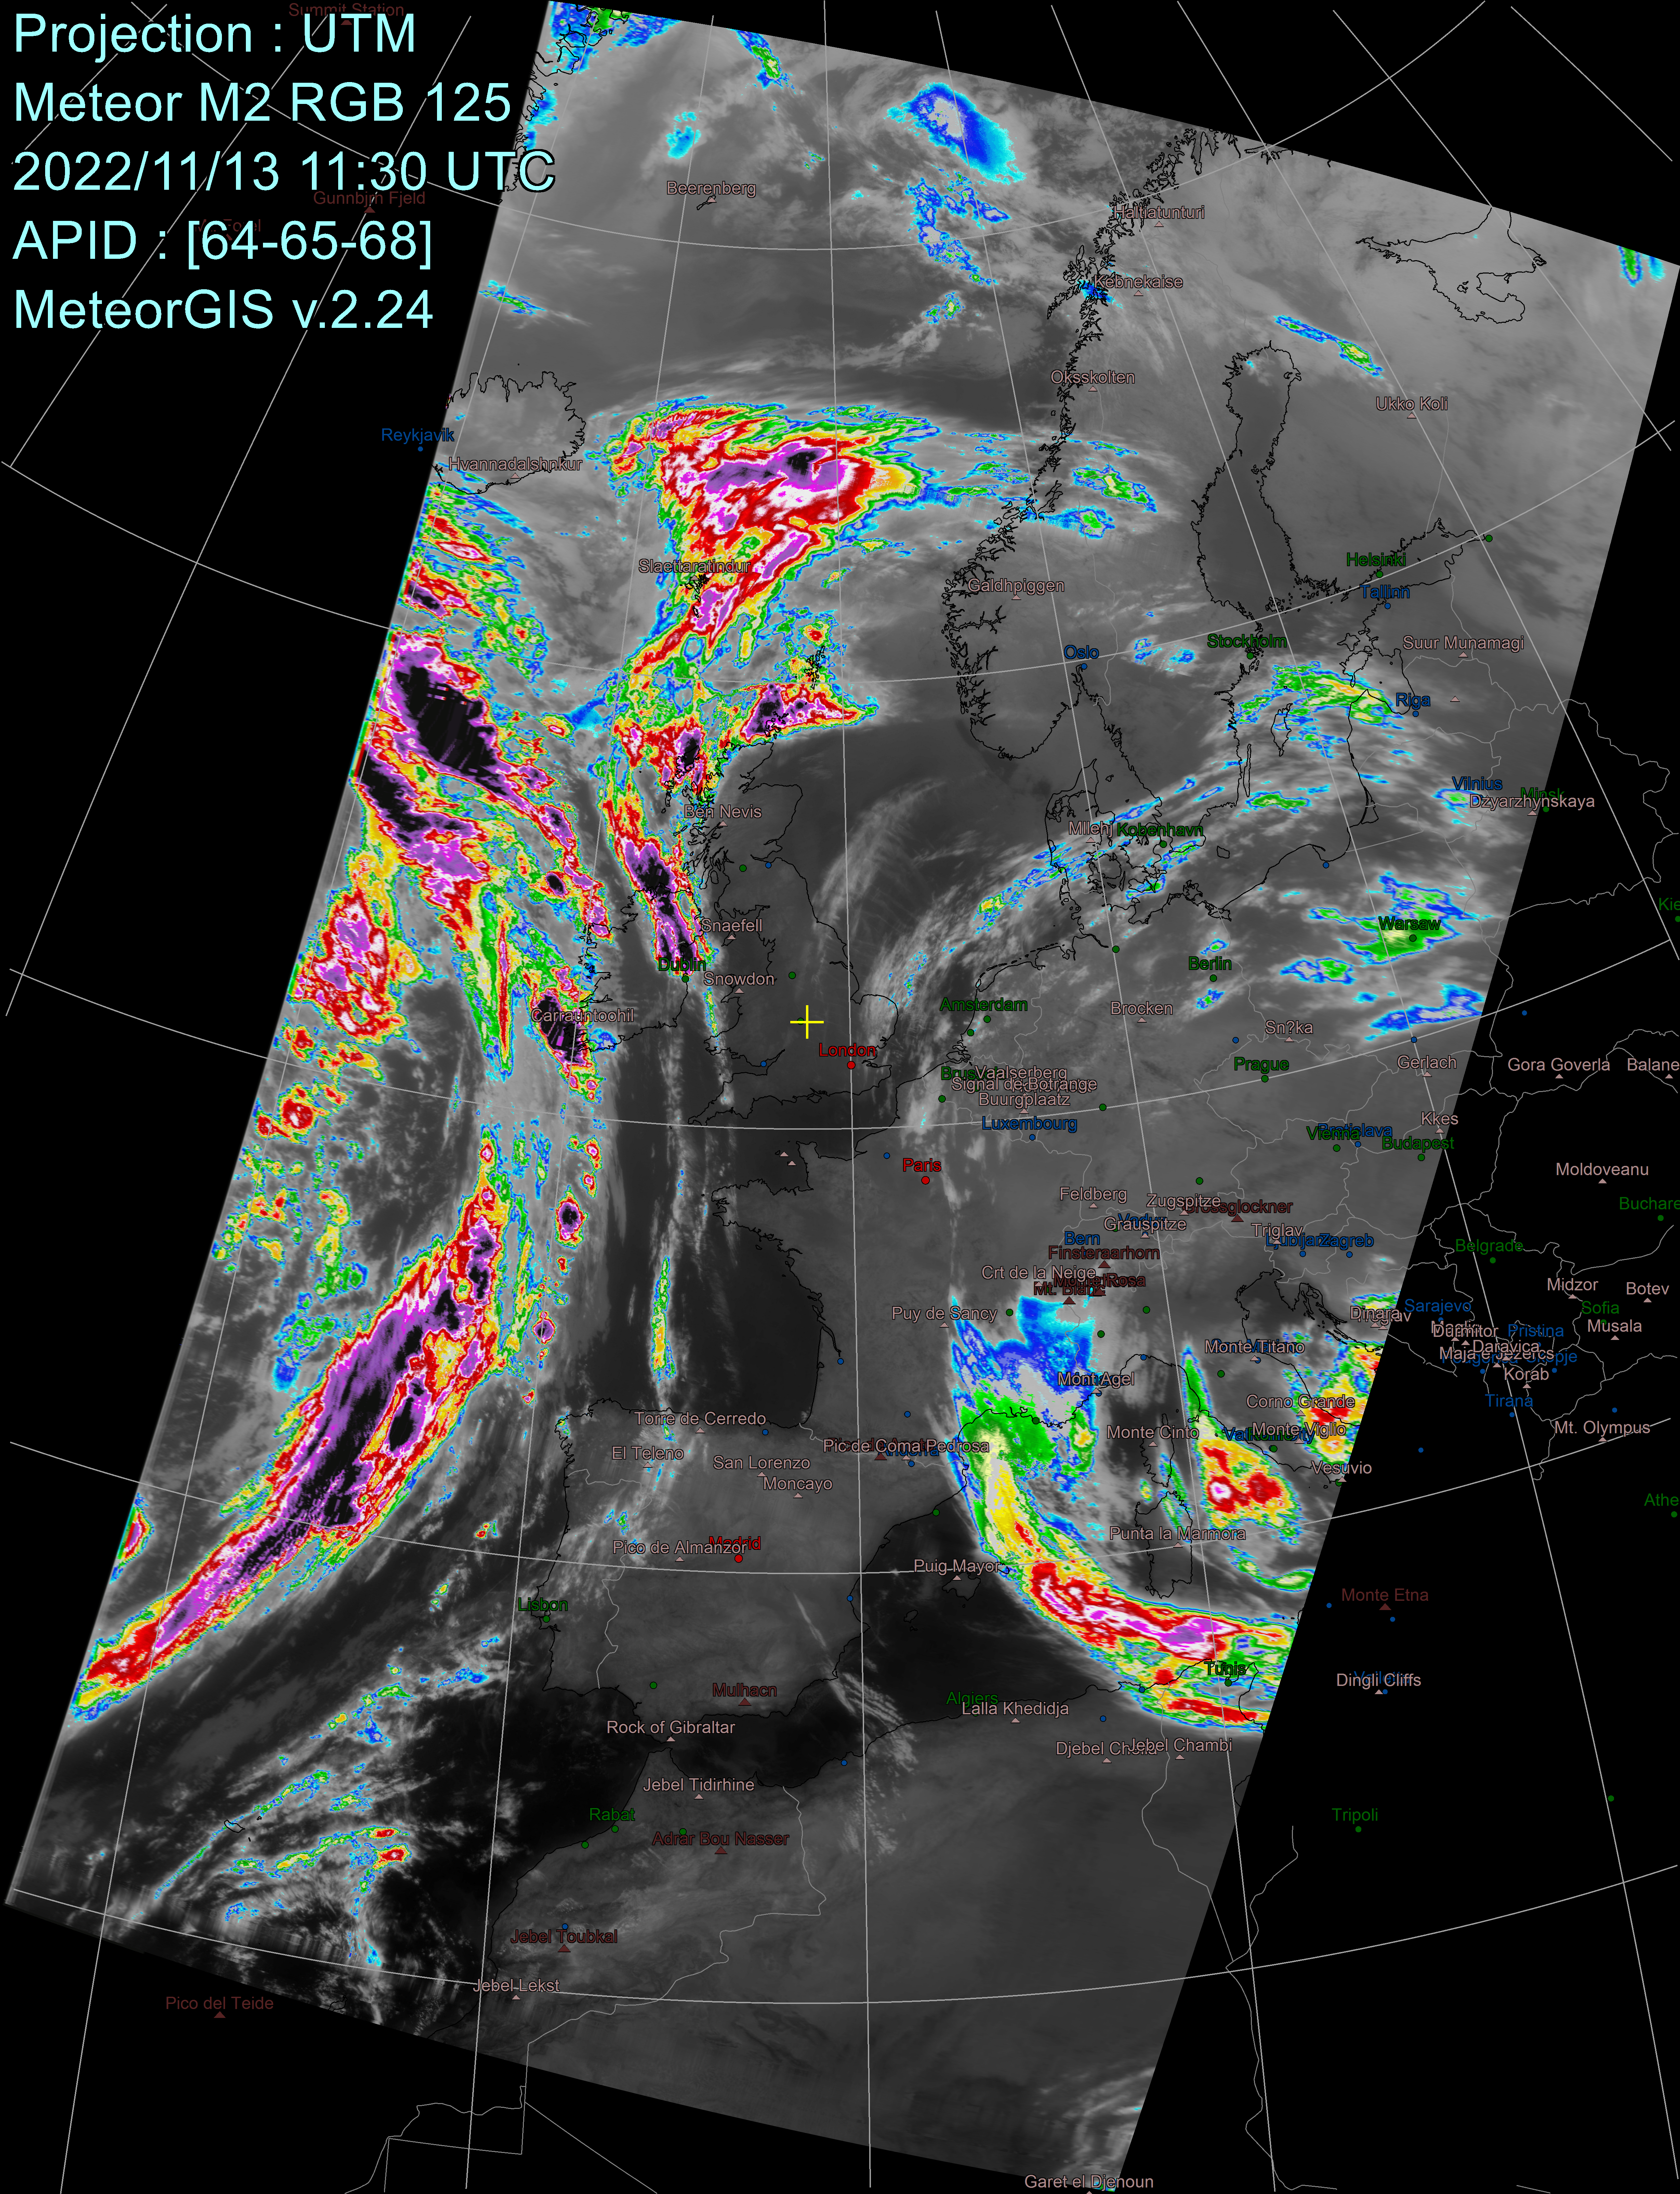
\includegraphics[scale=0.125]{imgs/UTM-2022-11-13-11-30-51-799_IR_rainfall(1).png}
                    \caption{Temperature composition of the UK region.}
                    \label{img:mount}
                \end{figure}  

            Such images could be used to predict the rainfalls as well as approaching cyclones. The data carried by the NOAA satellites however does not allow for such details like temperature, so for the weather prediction it is preferred to use METEOR satellites.
                
            \item[] Having captured 8 or so passes I was able to make a composite overlay of all the passes on one picture.

            \begin{figure}[H]
                    \centering
                    \includegraphics[scale=0.3]{imgs/compound.jpg}
                    \caption{Temperature composition of the UK region.}
                    \label{img:mount}
            \end{figure}  
            
        \end{itemize}
    \subsection{Possible improvements}
        \begin{itemize}
            \item[] Having made plenty of captures it became pretty clear that I was maxing out the possibilities of the APT and LRPT signals, the signal was clear and steady and the resulting images were clear. If I had more time and money, I would attempt to build a parabolic antenna for better pictures that same satellites transmit over the S-Band frequency (1.6 GHz). Higher frequency enables same satellite to encode more data in one sample, thus making it possible to transmit higher quality images. This approach would need a complete redesign of the antenna part as well as the receiver, because a parabolic antenna should always be pointed to the source of the signal -- satellite, unlike an omnidirectional V-Dipole design that I utilized throughout this project.
            \item[] If a couple of more people join the satellite data collection, the through collective effort we could build a composite map of the whole earth. Such projects already exits in the amateur radio community.
        \end{itemize}

\section{Conclusion}
    \begin{itemize}
        \item[] Having successfully built an affordable receiver setup, designed and implemented the antenna design, received and decoded a high resolution picture of earth surface, which could be used for weather predictions, I consider this project complete. I tried to keep the cost of the setup as low as possible and successfully selected the hardware which was both suitable for the purpose and quite comparatively cheap. This written report could be consequentially used as a guide for other amateurs to use. 
    \end{itemize}
    
\newpage

\section{References}
\begin{thebibliography}{9}

\bibitem{1}
https://www.futuretimeline.net/data-trends/6.htm  accessed 23/3/22

\bibitem{2}
https://www.washingtonpost.com/technology/2021/04/06/small-satellites-growth-space/  accessed 17/3/22

\bibitem{3}
https://www.esa.int/Enabling Support/Space Transportation/Types of orbits   accessed 17/3/22

\bibitem{4}
Kvamstad, Beate & Bekkadal, Fritz & Grythe, K. & Jensen, Irene Anite & Haakegaard, J.E. & Behlke, Rico. (2014). The MARENOR Project - Maritime Radio System Performances in the High North. 10.4043/24661-MS

\bibitem{5}
ZPhysics. (Sep 2, 2020). A Level Physics: Geostationary orbits, calculating the height of a geostationary orbit. [Video]. YouTube. https://youtu.be/DAAEW7TzBEY  accessed 19/3/22

\bibitem{6}
[Purcell and Morin, Harvard University. (2013). Electricity and Magnetism, 820p (3rd ed.). Cambridge University Press, New York. ISBN 978-1-107-01402-2. p 430

\bibitem{7}
https://www.5gtechnologyworld.com/digital-modulation-basics-part-1/  accessed 21/3/22

\bibitem{8}
https://www.elprocus.com/quadrature-phase-shift-keying-definition-with-circuit-diagram/  accessed 15/3/22

\bibitem{9}
https://mdahlem.net/astro/obs/radio/ovro.php  accessed 12/3/22

\bibitem{10}
https://www.researchgate.net/figure/The-structure-of-l-2-dipole-antenna-5 fig1 320751102  accessed 12/3/22

\bibitem{11}
https://terasense.com/terahertz-technology/radio-frequency-bands/  accessed 12/3/22

\bibitem{12}
https://www.researchgate.net/profile/Arno-Bouwens  accessed 17/3/22

\bibitem{13}
https://apbouwens.github.io/V-dipole-rad-pat/  accessed 18/3/22

\bibitem{14}
https://www.amazon.co.uk/RTL-SDR-RTL2832U-Software-Telescopic-Antennas\/dp\/B011HVUEME\/ref\=sr 13?keywords\=rtl\-sdr\&qid=1667741346\&sr=8-3   accessed 17/3/22

\bibitem{15}
https://www.rtl-sdr.com/rtl-sdr-quick-start-guide/  accessed 21/5/22

\bibitem{16}
https://leshamilton.co.uk/MeteorLRPTSuite.htm  accessed 21/5/22

\bibitem{17}
https://github.com/altillimity/SatDump  accessed 28/8/22

\bibitem{18}
https://github.com/rt-bishop/Look4Sat  accessed 29/2/22

\bibitem{19}
http://gpredict.oz9aec.net/

\end{thebibliography}


\section{Bibliography}
\begin{thebibliography}{9}
\bibitem{bib pass prediction}
Atkin, J.  [The Thought Emporium] (Mar 7, 2017) How to Pull Images from Satellites in Orbit (NOAA 15,18,19 and METEOR M2)Curtis, H.D. (2009) Orbital Mechanics for Engineering Students. 2nd Edition, Elsevier Ltd., Amsterdam.

\bibitem{bib ARPL}
Kvamstad, Beate & Bekkadal, Fritz & Grythe, K. & Jensen, Irene Anite & Haakegaard, J.E. & Behlke, Rico. (2014). The MARENOR Project - Maritime Radio System Performances in the High North. 10.4043/24661-MS

\bibitem{bib aviation}
Purcell and Morin, Harvard University. (2013). Electricity and Magnetism, 820p (3rd ed.). Cambridge University Press, New York. ISBN 978-1-107-01402-2. p 430

\bibitem{bib pysdr}
The ARRL Antenna book 24th ed. by American Radio Relay League (ARRL)

\textbf{Websites used:}

https://www.amazon.co.uk/RTL-SDR-RTL2832U-Software-Telescopic-Antennas/dp/B011HVUEME/ref=sr 1 3?keywords=rtl-sdr&qid=1667741346&sr=8-3  accessed 17/3/22

https://apbouwens.github.io/V-dipole-rad-pat/  accessed 18/3/22

https://www.elprocus.com/quadrature-phase-shift-keying-definition-with-circuit-diagram/  accessed 15/3/22

EO Sharing Earth Observation Resources [eoPortal Directory] Public Satellite Missions Catalogue. https://directory.eoportal.org/web/eoportal/satellite-missions/m/meteor-m-2 accessed 12/4/22

https://www.esa.int/Enabling Support/Space Transportation/Types of orbits   accessed 17/3/22

https://www.etti.unibw.de/labalive/experiment/qpsksignalgeneration/  accessed 19/5/22

https://www.5gtechnologyworld.com/digital-modulation-basics-part-1/  accessed 21/3/22 

https://www.faa.gov/about/officeorg/headquartersoffices/avs/offices/aam/cami/library/onlinelibraries /aerospace medicine/tu  accessed 6/5 22

https://www.futuretimeline.net/data-trends/6.htm  accessed 23/3/22

https://github.com/altillimity/SatDump  accessed 28/3/22 

https://github.com/rt-bishop/Look4Sat accessed 11/4/22

http://gpredict.oz9aec.net/ Alexandru Csete accessed 12/4/22

https://leshamilton.co.uk/MeteorLRPTSuite.htm  accessed 21/3/22

https://mdahlem.net/astro/obs/radio/ovro.php  accessed 12/3/22

https://www.ntia.doc.gov/files/ntia/publications/2003-allochrt.pdf accessed 1/4/22

https://www.researchgate.net/figure/The-structure-of-l-2-dipole-antenna-5 fig1 320751102  accessed 12/3/22

https://www.researchgate.net/profile/Arno-Bouwens  accessed 17/3/22

https://www.rtl-sdr.com/rtl-sdr-quick-start-guide/  accessed 21/3/22

SigIdWiki.com [Signal Identification Guide] Public signal identification pedia. https://www.sigidwiki.com

https://www.sigidwiki.com/wiki/Low Rate Picture Transmission (LRPT) accessed 21/3/22

https://terasense.com/terahertz-technology/radio-frequency-bands/  accessed 12/3/22

Lucas Teske (Feb 5, 2016) Recording NOAA APT Signals with GQRX and RTL-SDR on Linux. Personal Blog. https://lucasteske.dev/2016/02/recording-noaa-apt-signals-with-gqrx-and-rtl-sdr-on-linux/  accessed 17/3/22

https://www.vandijkenelektronica.nl/product/rtl-sdr-v3-tcxo-dongle-500khz-1700mhz-sma-aansluiting/ accessed 19/4/22

https://www.washingtonpost.com/technology/2021/04/06/small-satellites-growth-space/  accessed 17/3/22

Video YouTube. https://youtu.be/cjClTnZ4Xh4  accessed  2/3/22

Video https://www.youtube.com/watch?v=Q0qrU4nprB0  accessed  5/2/22

Daniel Vogelbacher (Dec 15, 2019) Receive METEOR weather satellite images with RTLSDR and GQRX on Linux. [Article]. Personal blog. https://blog.chaospixel.com/linux/2019/12/receive-meteor-satellite-images-with-rtlsdr-gqrx-linux.html  accessed 17/4/22

World Meteorological Organization [Observing Systems Capability Analysis and Review Tool – OSCAR] https://space.oscar.wmo.int/satellites  accessed 3/3/22

ZPhysics. (Sep 2, 2020). A Level Physics: Geostationary orbits, calculating the height of a geostationary orbit. [Video]. YouTube. https://youtu.be/DAAEW7TzBEY  accessed 19/3/2


\end{thebibliography}

\end{document}
